\begin{ZhChapter}

    \chapter{Implementation}
    The experimental implementation of this study is conducted on the Windows 11 operating system. Detailed configuration steps and set up instructions are described in the following subsection, including hardware and software requirements, environment set up and dataset preparation.


    \section{Hardware  and Software Requirements}
    \subsection{Environment Set up}
    Table \ref{table:hardware} provides detailed specifications of each hardware component utilized in our experimental environment and Table~\ref{tab:software} lists the software used in our experimental, along with their purposes and license types.

    \begin{table*}[htbp]
        \centering
        \caption{Hardware Requirements for the Experiment} \label{table:hardware}
        \makebox[\linewidth][c]{
            \renewcommand\arraystretch{1.2}{
                \begin{tabular}{| l | l |}
                    \hline
                    Component & Specification                                              \\
                    \hline
                    CPU       & 12th Gen Intel(R) Core(TM) i5-12500H @ 2.50 GHz            \\
                    RAM       & 16.0 GB (15.6 GB usable)                                   \\
                    Storage   & Built-in SSD (used for operating system and model storage) \\
                    \hline
                \end{tabular}
            }
        }
    \end{table*}

    \begin{table*}[htbp]
        \centering
        \caption{Software and Libraries Utilized in the Experiment} \label{tab:software}
        \vspace{1em}
        \makebox[\linewidth][c]{
            \renewcommand\arraystretch{1.2}{
                \begin{tabular}{| l | c | p{8cm} | c |}
                    \hline
                    Software/Library                 & Version & Purpose                                                                                                                                                    & License        \\
                    \hline
                    Ubuntu~\cite{ubuntu}             & 24.04.2 & Operating system                                                                                                                                           & MIT            \\
                    \hline
                    Python~\cite{python}             & 3.9.18  & The main programming language used to implement the core modules of the proposed system, including preprocessing, model training, and evaluation routines. & Python License \\
                    \hline
                    NumPy~\cite{numpy}               & 1.26.4  & Provides high-performance array structures and functions for numerical computing, especially efficient vector and matrix operations.                       & BSD            \\
                    \hline
                    Pandas~\cite{pandas}             & 2.2.2   & Offers powerful data manipulation and analysis tools, including DataFrame structures used for preprocessing and filtering packet data.                     & BSD            \\
                    \hline
                    Scikit-learn~\cite{scikit-learn} & 1.4.2   & Provides a wide range of machine learning algorithms, particularly the Multi-Layer Perceptron (MLP) classifier used in this study.                         & BSD            \\
                    \hline
                    mmh3~\cite{senuma2025mmh3}       & 4.0.1   & Implements MurmurHash3, a fast non-cryptographic hashing function used to convert tokens into integer values for embedding.                                & MIT            \\
                    \hline
                    PyTorch~\cite{imambi2021pytorch} & 2.2.2   & A deep learning framework used to define and train neural networks, including custom embedding and classification models.                                  & BSD            \\
                    \hline
                \end{tabular}
            }
        }
    \end{table*}


    \newpage
    \subsection{Environment Setup}
    This section will mainly introduce the installation procedures and environment setup required for the Structured Semantics and Generation Embedded Network Intrusion Detection System (S2GE-NIDS). To ensure dependency management and maintain an isolated environment, Python virtual environments must be set up first. The intallation steps are listed below:

    1. Install Ubuntu

    Before experiment,  it is necessary to install Ubuntu (as shown in Figure~\ref{fig:Ubuntu}) Download the Ubuntu of version 24.04 on the official website.\\

    After confirming the installation, you can confirm the current version as below.

    \begin{verbatim}
    cat /etc/os-release
    \end{verbatim}
    \begin{figure*}[htbp]
        \centering
        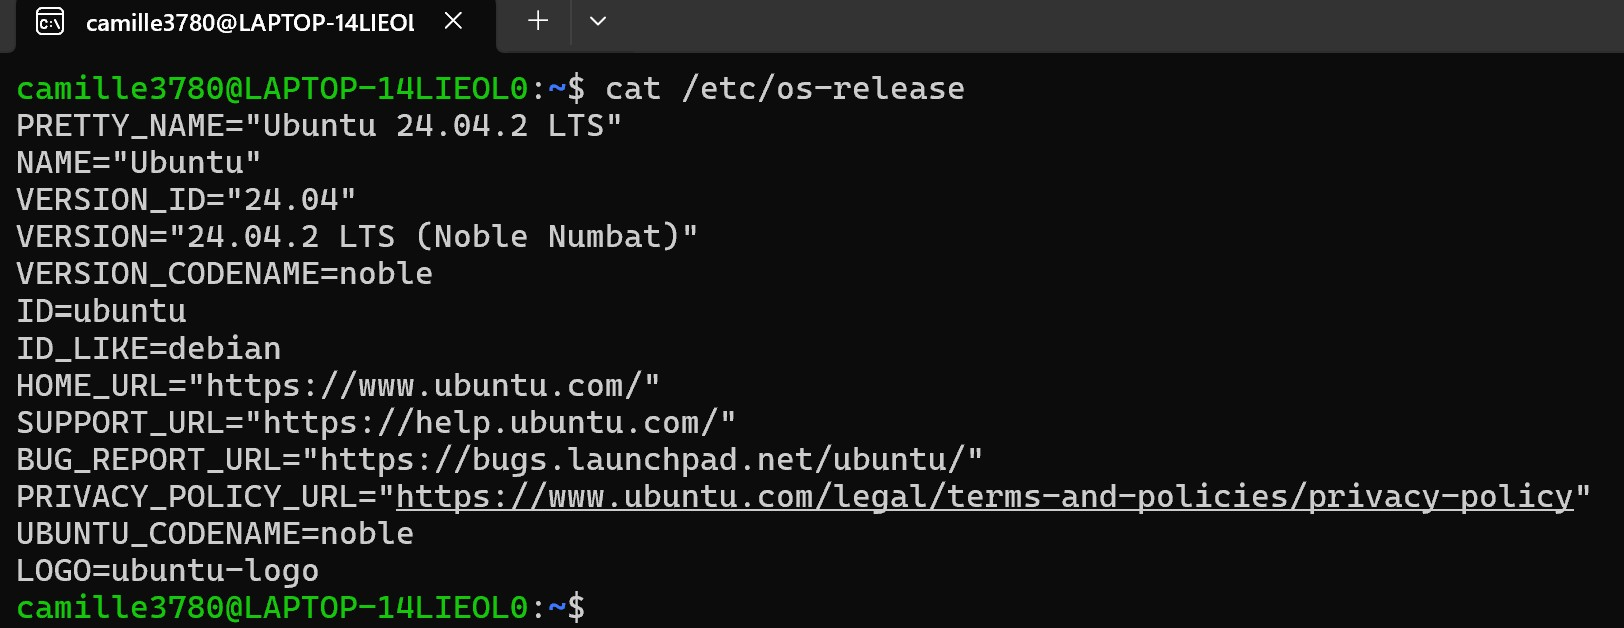
\includegraphics[width = 0.6\textwidth]{image/Ubuntu.jpg}
        \caption{Installation Procedure of the Ubuntu Operating System Environment}
        \label{fig:Ubuntu}
    \end{figure*}

    2. Install Python

    Download the Python package on the office website, (see Figure~\ref{fig:Python}) for this study.

    \begin{figure*}[htbp]
        \centering
        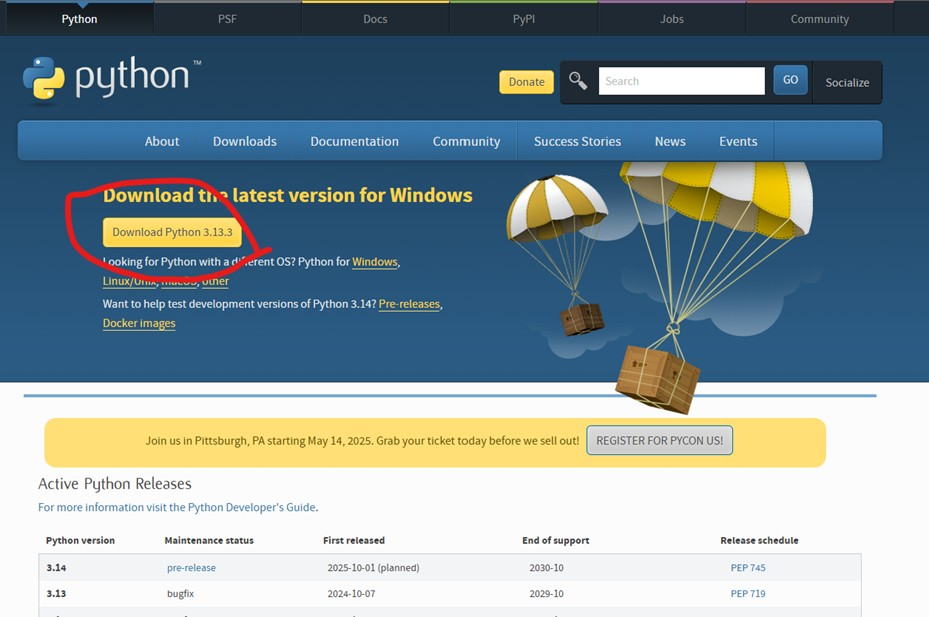
\includegraphics[width = 0.4\textwidth]{image/python.jpg}
        \caption{Installation Procedure of the Python Package}
        \label{fig:Python}
    \end{figure*}

    \newpage
    3. Activate the pre-configured virtual environment
    To use the S2GE environment, this command will be used to enable it.
    \begin{verbatim}
    python3 -m venv ~/nids_env
    source ~/nids_env/bin/activate
    \end{verbatim}




    Upon successful activation, the shell will displayed with \texttt{nids-env}, indicating that the virtual environment is active



    Figure~\ref{fig:Nids} shows how to enable virtual environment.

    \begin{figure*}[htbp]
        \centering
        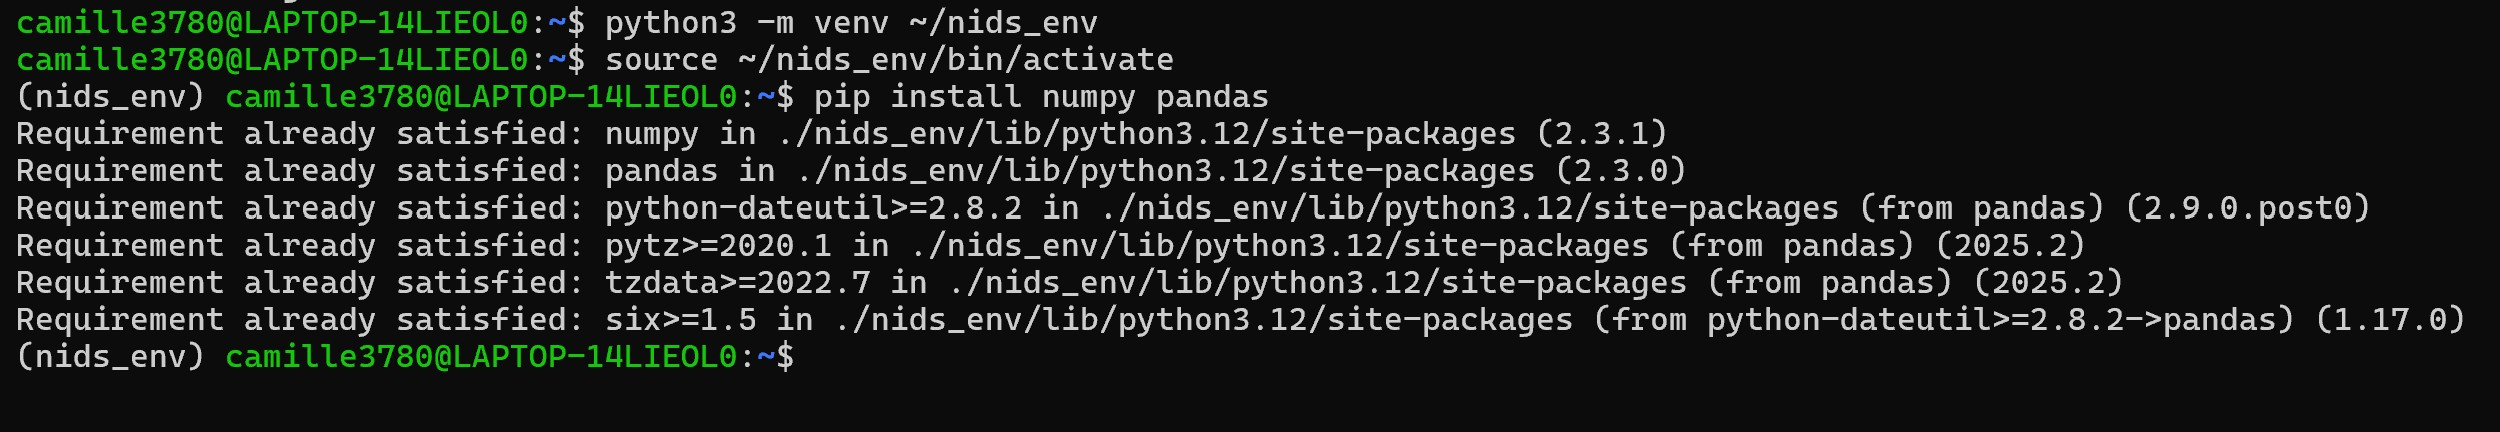
\includegraphics[width = 1\textwidth]{image/Nids-env.jpg}
        \caption{Setup of an Independent Python Virtual Environment}
        \label{fig:Nids}
    \end{figure*}




    4. Installing required packages
    \begin{verbatim}
    sudo apt install -y python3 python3-pip python3-venv build-essential
    pip install \
    numpy==1.26.4 \
    pandas==2.2.2 \
    scikit-learn==1.4.2 \
    mmh3==4.0.1 \
    torch==2.2.2+cpu \
    matplotlib seaborn

    \end{verbatim}






    \subsection{Data Preparation}
    In this experiment utilizes the latest 2024 Internet of Things (IoT) dataset~\cite{ciciot2024} as the source of experimental data. The dataset contains different network packet data collected from various smart devices operating in real-world environments, including both normal traffic and diverse abnormal behaviors, effectively reflecting the security threats and anomaly patterns faced by IoT systems. With a large volume of data and complete annotations, the dataset provides rich traffic features such as packet size, communication protocol types, source and destination IPs, making it suitable for training and testing anomaly detection models. By leveraging this dataset, this study aims to validate the applicability and effectiveness of the proposed method across diverse IoT device environments and enhance the model's capability to identify anomalies in real-world scenarios. The experimental results will be presented and analyzed in detail in the following chapter.


    This experiment uses CUDA to GPU acceleration for model training, and the training process executes 10 epochs in total.
    \begin{figure*}[!t]
        \centering
        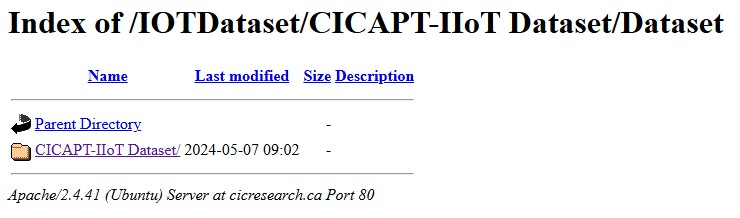
\includegraphics[width = 0.6\textwidth]{image/Dataset.jpg}
        \caption{Download the CIC IoMT dataset 2024}
        \label{fig:D}
    \end{figure*}



\end{ZhChapter}